%=======================
%velikost

\chapter{Techniky pro omezení velikosti}
Jak již bylo v úvodu řečeno, velikost aplikace je u inter důležitá.
Technik pro zmenšení výsledné aplikace je několik.
Je to nastavení překladače tak, aby odstranil všechna ne\-po\-u\-ží\-va\-ná data, a aby svůj překlad optimalizoval na výslednou velikost.
Dalším způsobem je výslednou aplikaci zkomprimovat speciálními balícími programy - takzvanými Exe packery.
Ty aplikaci zkomprimují a vloží na začátek algoritmus rozbalení a spuštění.
Další úsporu místa lze dosáhnou zvoleným jazykem a vhodnými konstrukcemi v něm.
Velmi důležitou část také tvoří generování grafického obsahu, protože nemůžeme mít uložena prakticky žádná data.
Mezi ostatní metody zmenšování velikosti programu patří obfuskace kódu, který je uložen ve statických datech a volba platformy, na které má aplikace běžet (rozdíl ve velikostech aplikace lze pozorovat u třiceti dvou bitových a šedesáti čtyř bitových verzích systému).

\section{Nastavení překladače}
Pro překlad této práce byl použit program GCC.
Ten umožňuje několik nastavení pro zmenšení velikosti.
Významné parametry jsou:
\begin{description}
\item[Parametr -s]
Kompilátor při využití tohoto parametru zahodí veškerý nevyužívaný kód programu.
Pokud se v programu vyskytne kód nebo data na které není odkazováno, nemají význam pro běh aplikace.
Parametr také zajistí odstranění všech statických údajů pro ladění programu.
Tyto údaje jsou například názvy funkcí a procedur.
Proto je vhodné tento parametr nepoužívat při ladění.
Tento parametr může výslednou velikost zmenšit i na třicet procent původní velikosti.

\item[Parametr -Os]
Tento parametr donutí kompilátor optimalizovat kód přeuspořádáním a hledáním výhodnějších konstrukcí.
Příkladem může být spojení dvou po sobě jdoucích cyklů se stejným počtem opakování.
Díky tomuto parametru může kompilátor obě smyčky spojit dohromady.
Nesmí však dojít ke změně významu.
Využitím tohoto parametru se aplikace může zmenšit až o několik stovek bajtů.

\item[Parametr -nostdlib]
Tento parametr odstraní veškeré standardní knihovny z aplikace a zanechá jenom nutné minimum.
Parametr se obvykle neobejde bez dalšího parametru: {\it-Wl,-emain}, kterým se specifikuje vstupní bod aplikace.
Nesmíme zapomenout, že aplikováním tohoto parametru se nám znepřístupní většina běžně používaných funkcí jako je například alokace paměti.
Proto je nutné tyto chybějící funkce dopsat a to obvykle v inline assembleru.
Příkladem funkce, kterou je nutné dopsat v inline assembleru je funkce exit, bez které se program neukončí korektně.
Využitím parametru je možné aplikaci zmenšit i o 5KB, nicméně toto zmenšení sebou přináší řadu ne\-pří\-jem\-nos\-tí v podobě nutného dopsání základních funkcí.
\end{description}

\section{Exe packer}
Exe packer je aplikace na komprimování zkompilovaných programů.
Výsledkem jeho aplikování je komprimovaný spustitelný soubor.
Těchto komprimační programů existuje ně\-ko\-lik.
Liší se svými algoritmy pro kompresi.
Některé pracují jen v některých operačních systémech a některé jsou multiplatformní.
Úzce zaměřené poskytují většinou větší komprimační poměr.

Mezi významnější komprimační programy patří UPX \cite{UPX} ve verzi 3.08.
Tento program je multiplatformní a jsou k dispozici jeho zdrojové kódy.
Tím, že je multiplatformní jej lze s výhodou použít pro multiplatformní intra.
Tímto komprimačním programem lze mimo spustitelné aplikace komprimovat i dynamicky linkované knihovny.
Poskytuje menší komprimační poměr.
Vytvářený program může zkomprimovat i na třicet procent jeho původní velikosti.

Další komprimační program se jmenuje kkrunchy \cite{KKRUNCHY}.
Tento exe packer vyvinula německá skupina Farbrausch.
Program běží v operačním systému Windows 7 a poskytuje jeden z nejlepších komprimačních poměrů.
Proto bývá často využívám při tvorbě inter.
Nastavením parametru při spuštění programu lze zvolit požadovanou výslednou velikost.

\section{Programátorský styl a konstrukce}
Vhodným programátorským stylem lze ušetřit také nějaké místo.
Existuje několik vý\-hod\-ných konstrukcí, které jsou v této práci používány:
\begin{itemize}
\item
Využívání funkcí.
Vhodné je často využívat funkce na části programu, které se opakují.
Toto patří k dobrému programátorskému stylu jako způsob dekompozice problému.
Nicméně, dobrým návrhem a hledáním míst programu, které lze sloučit do funkce lze dosáhnout zmenšení kódu i o stovky bajtů.
Důležité je dbát na to, aby se velikost aplikace zmenšila.
Nevhodným použitím funkcí může velikost naopak narůst.
Pokud máme jen několik řádků kódu, které používáme na mnoha místech (například sčítání dvou dvojrozměrných vektorů), nemusí mít vytváření funkce pro tyto řádky z pohledu velikosti smysl.
Volání funkce pro sečtení dvou vektorů může samo o sobě zabírat více místa.
Proto je výhodnější dané řádky kódu neobalovat funkcí.
Dobré z pohledu velikosti tak čitelnosti může být využití preprocesoru či inline funkcí, které se na místě volání rozbalí.

\item
Využití rekurze.
Programátorskou konstrukcí, která zmenšuje výslednou velikost je také rekurze.
Rekurze je sice pomalejší na vyčíslení, ale její vhodné použití může pomoci aplikace zmenšit.
Rekurze je zvláště vhodná pro procházení seznamů, zásobníků, front a stromů, kde se oproti řešení bez rekurze značně zmenšuje výsledná velikost algoritmů.

\item
Využití příkazu goto.
Příkaz goto (nepodmíněný skok) už většinou k dobrému programovacímu stylu nepatří.
Bývá doporučeno tento příkaz nevyužívat, kvůli zanesení nepřehlednosti do kódu.
Nicméně, pokud potřebujeme ušetřit i desítky bajtů, může být použití tohoto příkazu přínosné.
Výhodné je použít jej na vyskočení ze zanořené smyčky.
Další využití může být pro uvolňování paměti.
Uvažme případ, kdy si funkce v průběhu výpočtu alokuje na několika místech paměť.
Zároveň se funkce větví a může skončit na různých místech.
Před ukončením funkce je záhodné veškerou pomocnou alokovanou paměť uvolnit.
Vzhledem k tomu, že máme vícero ukončovacích míst, je nutné uvolnění dočasně alokované paměti provést na každém z nich, přičemž každé uvolnění se mírně liší.
Toto lze vyřešit vytvořením uvolňovací funkce.
Funkce bude mít tolik parametrů, kolik je proměnných k uvolnění.
Navíc uvolňovací funkce bude kontrolovat, zda je proměnná naplněná (proměnná nemusela být v daném ukončovacím místě původní funkce alokovaná).
Nevýhodou tohoto řešení je, že neušetří moc místa (pokud vůbec nějaké).
Další nevýhodou je, že uvolňovací funkce se využívá jen pro tuto funkci.
Výhodnější je na konec funkce uvést uvolnění proměnných v opačném pořadí něž jak jsou alokovány a za ně vložit jediný ukončovací bod funkce.
V místech, kde původní funkce končila se uvede příkaz goto na příslušné místo do uvolňovací sekvence.
Situace je znázorněna na obrázku \ref{fig:goto}.
\begin{figure}[h]
\centering
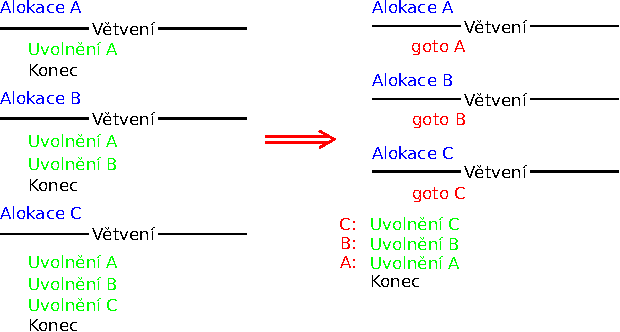
\includegraphics[width=15cm,keepaspectratio]{obr/goto.pdf}
\caption{Využití příkazu goto}
\label{fig:goto}
\end{figure}

\item
Vytýkání kódu.
Vytýkáním lze také ušetřit několik bajtů.
Vytknout lze (mimo jiné) také prolog a epilog části kódu.
Použití vytýkání epilogu můžeme vidět u příkladu využití goto znázorněného na \ref{fig:goto}.
O vytýkání kódu se snaží i kompilační program (při využití parametru {\it-s}), nicméně programátor má veškeré informace, tak tuto činnost dělá efektivněji.

\item
Rozbalení smyček.
U smyček jejichž tělo je dostatečně malé a počet opakování nízký, může vést rozbalení k uspoření místa.

\item
Obecné abstraktní datové typy.
Vytvořením obecných abstraktních datových typů, jako je například seznam, můžeme program také zmenšit.
V případě, kdy seznam potřebujeme na vícero místech, může být vytvoření obecného seznamu dobrým krokem.
Obecná implementace abstraktního datového typu obvykle zabere více místa než implementace konkrétní, avšak, pokud je tento typ využíván na vícero místech programu, může  být jeho použití výhodné.
Zmenšení velikosti totiž spočívá ve sdílení obslužných funkcí.

\item
Využívání bitových a jiných operací.
Části některých algoritmů lze efektivně zmenšit pomocí série operátorů.
Výsledkem je úspora místa za cenu přehlednosti.
Příkladem nechť je inicializace matice M na jednotkovou matici:
\begin{verbatim}
for(int i=0;i<16;++i)
  M[i] = i%4 == i/4;
\end{verbatim}

\item
Inline assembler.
Assembler se často využívá u malých inter, protože poskytuje velkou úsporu místa.
Jeho nevýhodou je však ztráta přehlednosti a do jisté míry i pře\-no\-si\-tel\-nos\-ti kódu.

\item
Jiné.
Mezi další techniky můžeme zařadit špatné programátorské návyky.
V případě, že se snažíme ušetřit každý bajt, se můžeme rozhodnout neuvolňovat námi alokovanou paměť a doufat, že potřebnou dealokaci provede operační systém.
Další možností je vytvoření vícero zkompilovaných verzí aplikace, a tím odstranit nutnost zpracování argumentů po spuštění (ve kterých může být například šířka a výška okna).

\end{itemize}

Při implementaci algoritmů pro intro se často setkáme se situací, kdy se musíme rozhodnout, mezi velikostí, rychlostí, znovupoužitelností a čitelností.
Všechny tyto vlastnosti jdou proti sobě až na čitelnost, kterou lze téměř vždy zajistit.
Záleží jen na situaci a schopnostech programátora předpovídat, která z implementací daného algoritmu je vhodnější.
Případně lze naprogramovat vícero variant, mezi kterými se v případě potřeby přepne preprocesorem.

\section{Šablony, generování grafického obsahu}
Bez generování grafického obsahu by se intra neobešla.
Generování a šablony jsou základem všech inter.
Díky generování obsahu podle šablon lze ušetřit nejvíce místa.
Lze ušetřit desítky i stovky megabajtů.
Namísto, aby se v aplikaci ukládaly textury a modely, uloží se jen způsob, jak je vytvořit.
Například nebudeme ukládá body kružnice, uložíme si jen poloměr a střed a algoritmus na vygenerování bodů kružnice.
Tento způsob uložení má několik výhod. První z nich je velikost, která je o mnoho menší.
Další výhodou je parametrizování generování.
Můžeme si zvolit kvalitu (počet bodů na kružnici), střed i poloměr.
Neuložili jsme si tedy jen jednu kružnici, ale všechny možné kružnice ve všech možných kvalitách a to s konstantní velikostí dat.
Výsledné intro lze tedy dobře parametrizovat a jen malými změnami parametrů markantně měnit grafický obsah.
Generování grafického obsahu je věnována celá kapitola \ref{chap:generovani}.

\section{Další techniky, obfuskace}
Mezi další techniky minimalizace velikosti patří obfuskace \cite{OBFUSKACE}.
Obfuskace je využití syntaxe jazyka tak, že se použijí co nejkratší textové konstrukce pro daný program.
Obvykle to zahrnuje odstranění komentářů, zkrácení identifikátorů a zrušení formátování.
Toto lze použít jen ve speciálních případech, kdy je program uložen nezkompilovaný ve statických datech.
Týká se to programů v jazyce GLSL.
U rozsáhlejších programů v GLSL (shaderech) lze dosáhnou úspory až stovek bajtů.
Nevýhodou obfuskace je absolutní ztráta čitelnosti.
%Obfuskaci lze použít i na programy v jazyce OpenCL.
